%=====================================================================
\section*{Question 4 -- Spatio-temporal traffic forecasting}

\subsection*{(a) Forecasting windows}
For every prediction time $t$ the input is $X_t=[x_{t-7},\dots,x_t]\in\R^{8\times716\times1}$ and the target is
$Y_t=[x_{t+1},\dots,x_{t+4}]\in\R^{4\times716\times1}$ (2\,h of history $\to$ the next 1\,h). Chronological splits on
the 15-min axis:
\begin{center}
\begin{tabular}{lll r}\toprule
Split & Period & 15-min steps & Windows\\\midrule
Train & 2020-01-01 -- 2020-12-31 & 35\,136 & 35\,125\\
Validation & 2021-01-01 -- 2021-03-31 & 8\,640 & 8\,629\\
Test & 2021-04-01 -- 2021-12-31 & 26\,400 & 26\,389\\\bottomrule
\end{tabular}
\end{center}
\begin{itemize}
\item \textbf{No window crosses a split boundary}: a window starting at $s$ uses steps $s,\dots,s+11$, and only
starts with \emph{both} input and target inside the same split are kept (hence 11 fewer windows than steps per split).
\item \textbf{Normalisation}: z-score with a single mean/std ($\mu=607.4$, $\sigma=483.8$ veh/15\,min) computed from
\emph{observed training} values only. Predictions are de-normalised before the loss, so the loss and all metrics are in
the original unit (vehicles per 15 min).
\item \textbf{Missing targets}: the loss (masked MAE) and MAE/RMSE are computed only over target entries that were
really observed; filled values are used only as inputs (Q3a).
\end{itemize}

\subsection*{(b) Architecture}
All models share the same three components (\texttt{src/models.py}); only $\hat A$ changes.
\begin{enumerate}
\item \textbf{Temporal encoder} $Z=f_{\text{temporal}}(X)\in\R^{B\times N\times d}$, $d=32$: the same 1D CNN is applied to
each sensor's 8-step series: Conv1d$(1\!\to\!32,k{=}3)$--ReLU--Conv1d$(32\!\to\!32,k{=}3)$--ReLU--Conv1d$(32\!\to\!32,k{=}4)$--ReLU.
The time axis shrinks $8\to6\to4\to1$, so the last layer summarises the whole 2-hour window into one $d$-vector per sensor.
\item \textbf{Graph convolution} $H=\mathrm{ReLU}(\hat A Z W_g)$, implemented as
\texttt{einsum("nm,bmd->bnd", A, W(z))}: the multiplication runs over the node axis, independently for each batch item.
\item \textbf{Forecast head} MLP Linear$(32\!\to\!32)$--ReLU--Linear$(32\!\to\!4)$ applied per sensor, giving
$\hat Y\in\R^{B\times4\times N\times1}$.
\end{enumerate}
Training: masked MAE loss, Adam (lr $10^{-3}$, weight decay $10^{-4}$), batch 64, gradient clipping at 5,
ReduceLROnPlateau (factor 0.5, patience 3), at most 50 epochs with early stopping on validation MAE (patience 8); the
best-validation checkpoint is evaluated on the test set. Seed 42 for Python, NumPy and PyTorch, cuDNN deterministic.
The validation and test MAE/RMSE for every model are in Table~\ref{tab:main} (Q6a).

\noindent\textbf{Skip-connection variant.} Following the result in Q3(c) that aggregation can erase a sensor's own
information, every model was also trained with a single change: the head receives $Z+H$ instead of $H$
(\texttt{--residual}). Everything else (encoder, head, splits, protocol, seed) is identical. Both variants are reported.

\subsection*{(c) Temporal-only baseline}
The baseline uses the same encoder, the same $W_g$ layer and the same head, but $\hat A=I$: each sensor only sees its
own encoding, so there is no message passing between sensors. It therefore has exactly the same parameter count (9\,604)
as the fixed-graph STGNN, and any difference is due to spatial aggregation alone.

\begin{center}
\begin{tabular}{l cc cc}\toprule
& \multicolumn{2}{c}{as specified (head sees $H$)} & \multicolumn{2}{c}{with skip (head sees $Z{+}H$)}\\
\cmidrule(lr){2-3}\cmidrule(lr){4-5}
Model & Test MAE & Test RMSE & Test MAE & Test RMSE\\\midrule
Temporal-only ($\hat A=I$) & \textbf{64.75} & \textbf{102.40} & 64.57 & 101.81\\
STGNN, fixed road graph & 142.19 & 221.80 & \textbf{59.80} & \textbf{94.26}\\\bottomrule
\end{tabular}
\end{center}
\textbf{Does modelling spatial dependencies help?} It depends on how the spatial information is combined:
\begin{itemize}
\item \textbf{As specified, no; it is much worse} (MAE $64.8\to142.2$). With the directed row normalisation the self-weight
of sensor $i$ is $1/\sum_j\tilde A_{ij}$ (median 0.14), so about 86\% of $H_i$ comes from neighbours, and the head has no other
access to $Z_i$. Neighbouring sensors can have very different volumes (an on-ramp next to a 6-lane mainline,
flow levels differ by $10\times$ across the network), so the model predicts the neighbourhood's level, not the sensor's. Fig.~\ref{fig:pred1}
shows this: for sensor 1118170 the fixed-graph model overshoots the weekday peaks by several hundred vehicles per 15 min. The error is almost
the same at every horizon (135 at 15\,min, 150 at 60\,min, Table~\ref{tab:horizon}), i.e.\ it is a level bias, not a dynamics error.
\item \textbf{With the sensor's own features kept, yes.} The fixed graph then reduces test MAE by 7.4\% (64.6 $\to$ 59.8) and RMSE by
7.4\%, and the gain grows with the horizon (4.5\% at 15\,min, 8.8\% at 60\,min). This is what the Q3(c) argument predicts:
a sensor's own past is enough for the next 15 minutes, but 30--60 minutes ahead, traffic arriving from upstream and
congestion spreading back from downstream (visible only at neighbours) become informative.
\end{itemize}
So spatial dependencies do improve accuracy, but only when the graph layer \emph{adds} neighbour information to the node's
own representation instead of replacing it.

%=====================================================================
\section*{Question 5 -- Fixed versus learnable adjacency}

\subsection*{(a) Fixed adjacency: directed normalisation}
$A_{SD}$ is not symmetric (Q3b), so $D^{-1/2}(A{+}I)D^{-1/2}$ (which needs one degree per node) does not apply directly. I use the
\textbf{directed random-walk normalisation}
\[
\hat A_{\text{fixed}}=D_{\text{out}}^{-1}\tilde A,\qquad \tilde A=A \text{ with } \tilde A_{ii}=1,\qquad
(D_{\text{out}})_{ii}=\textstyle\sum_j\tilde A_{ij}.
\]
\begin{itemize}
\item LargeST's adjacency already has $A_{ii}=1$, so the diagonal is \emph{set} to 1 rather than adding $I$ (which would give
self-loops of weight 2).
\item Row $i$ of $\hat A$ is a weighted \emph{average} over $i$ and the sensors it has an edge to, with the edge direction kept
($H_i$ uses row $i$, i.e.\ the sensors reachable from $i$). Every row sums to 1, so the scale of $H$ does not depend on the degree, and
the three isolated sensors simply keep their own features.
\item It is row-stochastic like the softmax-normalised adaptive matrix, so both can be combined consistently in Q5(c).
\end{itemize}
$\hat A_{\text{fixed}}$ is computed once and stored as a non-trainable buffer, so it stays unchanged throughout training.
Results (test): MAE 142.19 / RMSE 221.80, training time 337\,s as specified; MAE 59.80 / RMSE 94.26, 354\,s with the skip
connection (Table~\ref{tab:main}).

\subsection*{(b) Learnable adjacency}
\[
A_{\text{adaptive}}=\mathrm{Softmax}_{\text{row}}\big(\mathrm{ReLU}(E_1E_2^\top)\big),\qquad E_1,E_2\in\R^{716\times d_e},\ d_e=10,
\]
implemented directly in PyTorch (\texttt{AdaptiveAdjacency} in \texttt{src/models.py}, no library graph-learning layer).
$E_1$ and $E_2$ are initialised i.i.d.\ $\mathcal N(0,1/d_e)$ and trained jointly with the rest of the network by backpropagation
through the softmax and ReLU. Using two different matrices makes the learned graph directed ($E_1E_2^\top$ is not symmetric). The
matrix is recomputed at every forward pass (one $716\times716$ product, cheap on CPU as well).
\begin{itemize}
\item It is learned from the training loss only; validation and test data are never used to build it.
\item \textbf{Sparsification.} The reported runs use the \emph{dense} matrix ($N=716$ is small enough). The code supports top-$k$
(\texttt{--topk}): it is applied \textbf{before} normalisation, by setting every logit outside a row's $k$ largest to $-\infty$
and then applying the softmax, so each row is re-normalised over its $k$ kept neighbours. Gradients flow only through the
kept entries; the top-$k$ selection itself is piecewise constant (like an argmax) and has no gradient, but which entries
are kept can still change between steps as $E_1,E_2$ change.
\end{itemize}
The learned matrix is visualised in Fig.~\ref{fig:adj}. Compared with fixed adjacency, the adaptive graph is far better in the
as-specified setting (test MAE 79.75 vs 142.19) and also better with the skip connection (54.16 vs 59.80, $-9.4\%$; it is the best
model overall). Section Q6(b) analyses what it actually learned.

\subsection*{(c) Hybrid adjacency}
\[
A_{\text{hybrid}}=\lambda\,\hat A_{\text{fixed}}+(1-\lambda)\,A_{\text{adaptive}},\qquad \lambda=\sigma(\theta)\in(0,1),
\]
with $\theta$ a learned scalar initialised so that $\lambda=0.5$. Both matrices are row-stochastic (row normalisation and row softmax),
so they are on the same scale and the convex combination is again row-stochastic. Encoder, head, splits, protocol and seed are the
same as in (a) and (b).
\begin{itemize}
\item As specified: test MAE 78.92 / RMSE 124.40 (the best of the three graph models). $\lambda$ falls from 0.5 to \textbf{0.35}: the
model moves weight towards the learned graph but keeps a third on the road graph.
\item With skip: test MAE 54.20 / RMSE 86.31, the same as adaptive (54.16 / 86.23) within noise. Here $\lambda$ drops quickly to
\textbf{0.04} (Fig.~\ref{fig:lambda}): once the node's own features reach the head directly, the model almost switches the road graph off.
\end{itemize}
\begin{figure}[H]\centering
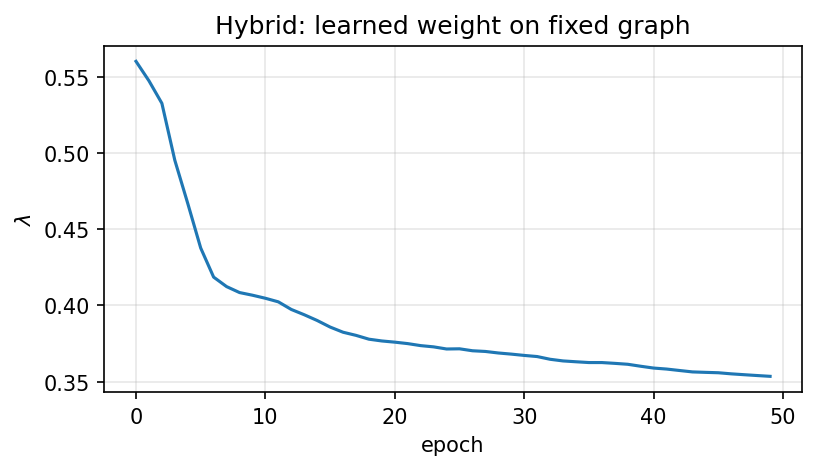
\includegraphics[width=.5\textwidth]{q5c_lambda.png}
\caption{Hybrid model (as specified): learned weight $\lambda$ on the fixed graph per epoch.}\label{fig:lambda}
\end{figure}

%=====================================================================
\section*{Question 6 -- Experimental analysis and interpretation}

\subsection*{(a) Forecasting comparison}
\begin{table}[H]\centering\small
\caption{Validation and test errors (vehicles per 15 min; average over the 4 horizons; observed targets only) and measured
training time on the GPU listed in Q7. Epochs: number run (best epoch). Upper block: the architecture exactly as specified;
lower block: same models with the skip connection. Best per block in bold.}\label{tab:main}
\resizebox{\textwidth}{!}{%
\begin{tabular}{llrrrrrrc}\toprule
Model & Adjacency & Val MAE & Val RMSE & \textbf{Test MAE} & \textbf{Test RMSE} & Params & Train time & Epochs\\\midrule
\multicolumn{9}{l}{\emph{as specified: head sees $H$}}\\
Temporal-only & None     & \textbf{56.20} & \textbf{90.93} & \textbf{64.75} & \textbf{102.40} & 9\,604 & 316\,s & 50 (46)\\
STGNN & Fixed            & 125.81 & 202.70 & 142.19 & 221.80 & 9\,604 & 337\,s & 50 (49)\\
STGNN & Adaptive         & 65.11 & 112.53 & 79.75 & 127.71 & 23\,924 & 359\,s & 50 (48)\\
STGNN & Hybrid           & 64.94 & 110.16 & 78.92 & 124.40 & 23\,925 & 367\,s & 50 (50)\\\midrule
\multicolumn{9}{l}{\emph{with skip connection: head sees $Z+H$}}\\
Temporal-only & None     & 55.65 & 89.69 & 64.57 & 101.81 & 9\,604 & 345\,s & 50 (48)\\
STGNN & Fixed            & 51.29 & 82.76 & 59.80 & 94.26 & 9\,604 & 354\,s & 50 (44)\\
STGNN & Adaptive         & \textbf{45.42} & \textbf{73.60} & \textbf{54.16} & \textbf{86.23} & 23\,924 & 356\,s & 48 (40)\\
STGNN & Hybrid           & 45.67 & 74.16 & 54.20 & 86.31 & 23\,925 & 377\,s & 50 (48)\\\bottomrule
\end{tabular}}
\end{table}

\begin{table}[H]\centering\small
\caption{Test MAE per forecast horizon.}\label{tab:horizon}
\begin{tabular}{ll rrrr rrrr}\toprule
& & \multicolumn{4}{c}{as specified} & \multicolumn{4}{c}{with skip}\\\cmidrule(lr){3-6}\cmidrule(lr){7-10}
Model & Adjacency & 15\,min & 30\,min & 45\,min & 60\,min & 15\,min & 30\,min & 45\,min & 60\,min\\\midrule
Temporal-only & None & 44.7 & 58.7 & 71.3 & 84.3 & 44.6 & 58.5 & 71.1 & 84.1\\
STGNN & Fixed        & 135.1 & 139.5 & 144.4 & 149.9 & 42.6 & 54.5 & 65.4 & 76.7\\
STGNN & Adaptive     & 74.2 & 77.7 & 81.4 & 85.7 & 40.3 & 50.2 & 58.9 & 67.3\\
STGNN & Hybrid       & 73.2 & 76.6 & 80.4 & 85.5 & 40.5 & 50.2 & 58.9 & 67.1\\\bottomrule
\end{tabular}
\end{table}

\noindent\textbf{Observations.}
\begin{itemize}
\item The test error is higher than the validation error for every model (about +9 MAE for most). Errors scale with the flow level, and the
test period (Apr--Dec 2021) carries more traffic: mean observed flow 721, vs 635 in Jan--Mar 2021 and 607 veh/15\,min in 2020
(training). All models are evaluated on the same test windows, so the comparison is fair.
\item Training times differ by less than 20\% (316--377\,s for 50 epochs, 6.3--7.5\,s/epoch). The adaptive graph adds a dense
$716\times716$ matrix product per step but no noticeable cost at this size.
\item Most runs reached their best validation score near epoch 50 (Fig.~\ref{fig:curves}), so a longer budget would lower all errors
slightly; the adaptive and hybrid models with skip (54.16 vs 54.20) are too close to rank.
\item The adaptive and hybrid models have 14\,320 more parameters ($2\times716\times10$ embeddings) than fixed, which is part of their
advantage.
\end{itemize}

\begin{figure}[H]\centering
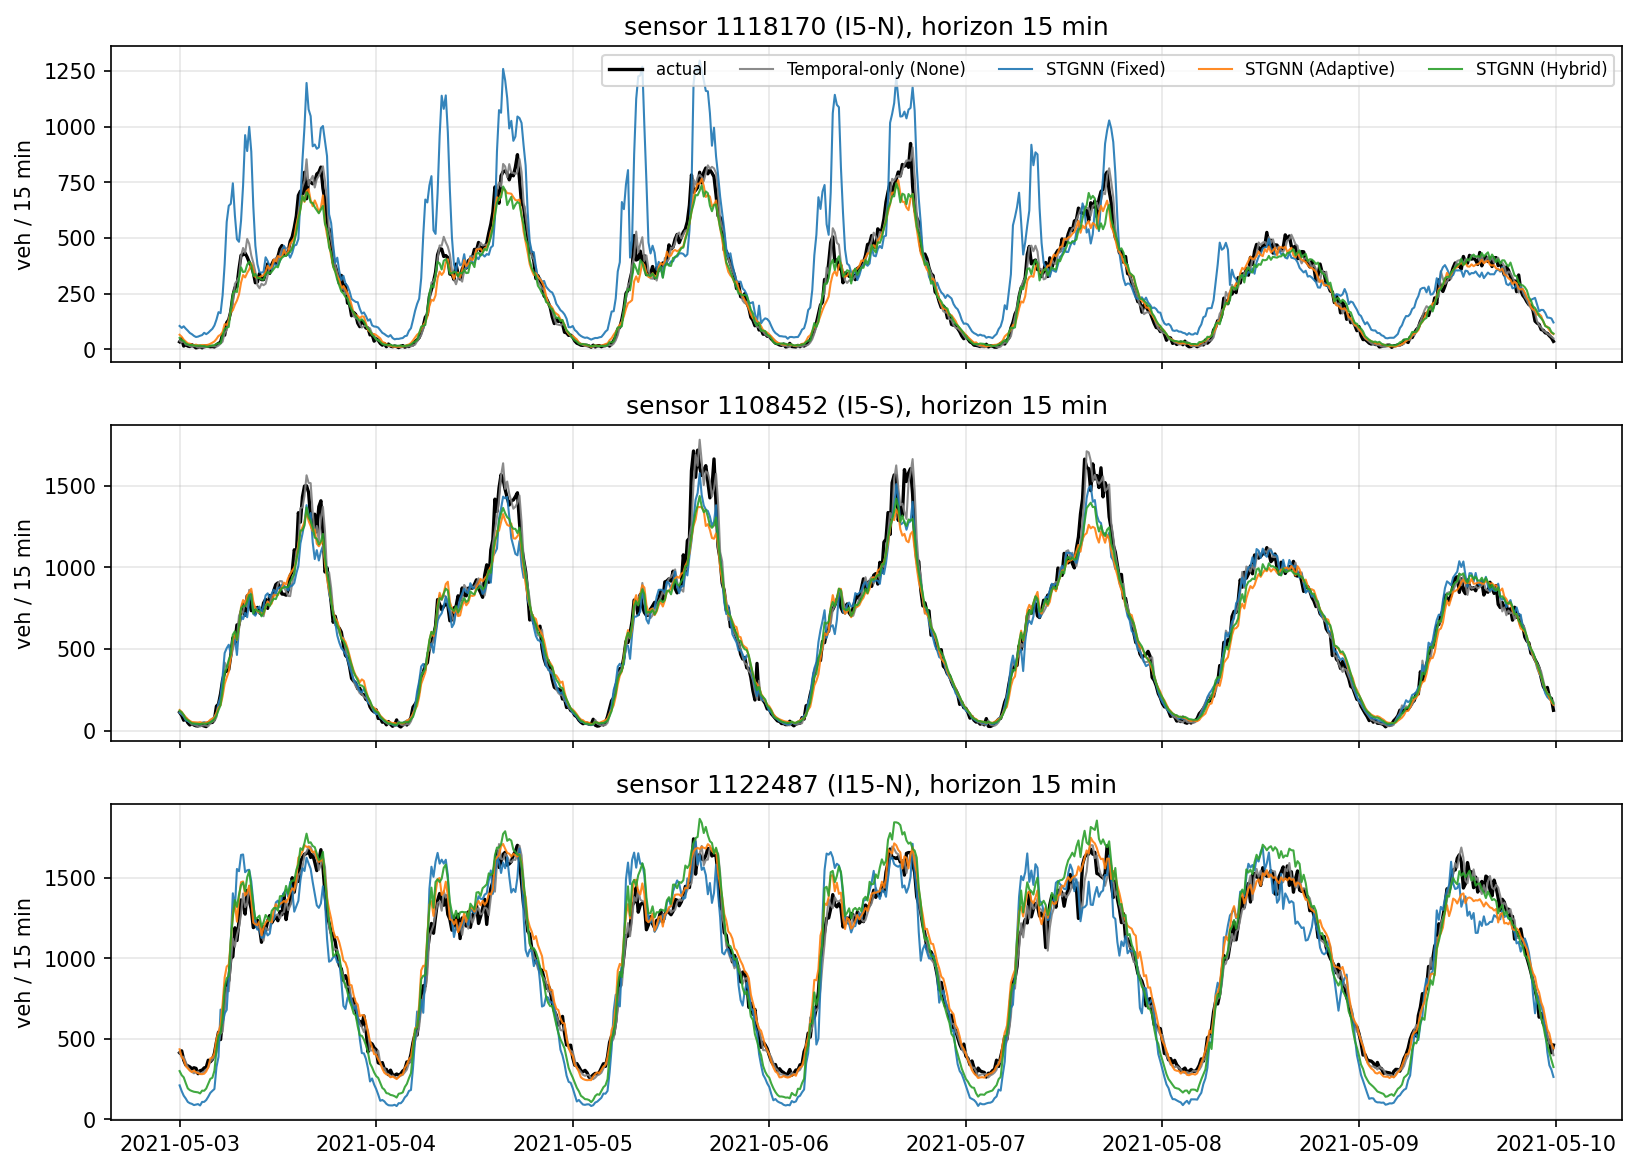
\includegraphics[width=.95\textwidth]{q6a_pred_vs_actual_h1.png}
\caption{Predicted vs.\ actual flow, 15-min horizon, architecture as specified, one test week (3--9 May 2021), three sensors on
I-5 N, I-5 S and I-15 N. The fixed-graph model (blue) overshoots the peaks at sensor 1118170 and undershoots night-time flow at
1122487: it predicts the level of the neighbourhood.}\label{fig:pred1}
\end{figure}
\begin{figure}[H]\centering
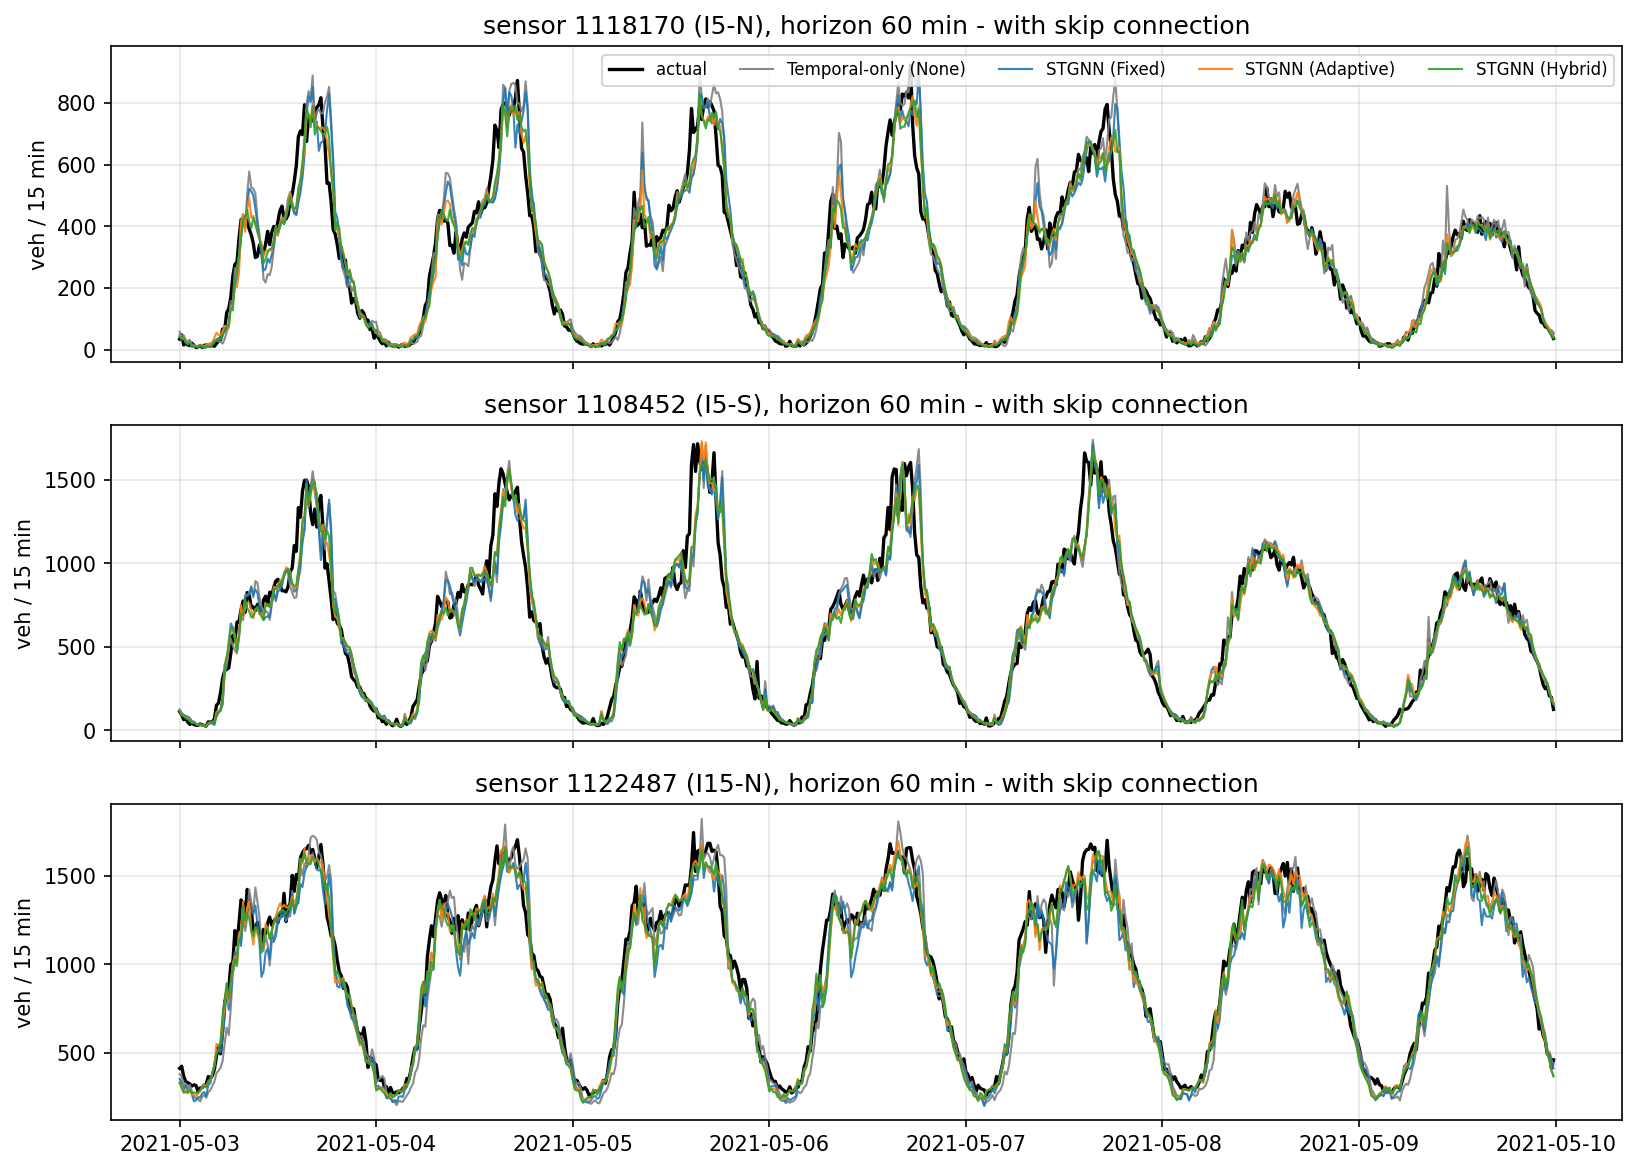
\includegraphics[width=.95\textwidth]{q6a_pred_vs_actual_res_h4.png}
\caption{Predicted vs.\ actual flow, 60-min horizon, models with skip connection, same week and sensors. All graph models follow
the daily shape, the weekday/weekend difference and the PM peak; errors are mostly at sharp peaks and sudden drops.
Plots for the other horizon/variant combinations are in \texttt{figures/q6a\_pred\_vs\_actual*}.}\label{fig:pred2}
\end{figure}
\begin{figure}[H]\centering
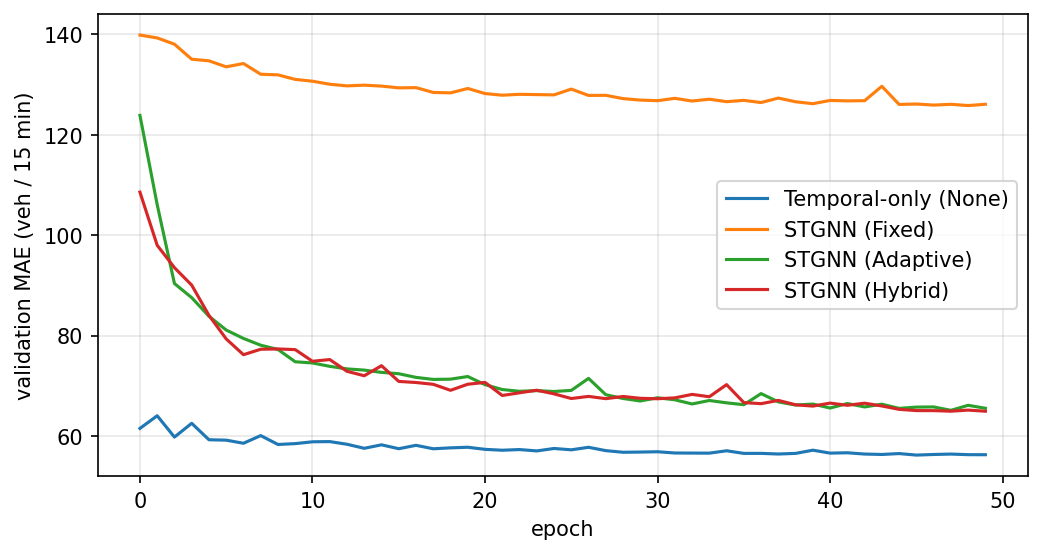
\includegraphics[width=.6\textwidth]{q6_val_curves.png}
\caption{Validation MAE per epoch, architecture as specified.}\label{fig:curves}
\end{figure}

\subsection*{(b) Graph structure analysis}
For each sensor $i$ I take the 10 largest off-diagonal entries of row $i$ of the learned $A_{\text{adaptive}}$ (7\,160 edges) and compare
them with the road graph, straight-line distances and the training-period correlation of de-seasonalised 15-min changes
(Q3c). The last column of Table~\ref{tab:graph} gives references: random pairs, or the road graph itself. (\texttt{results/q6b\_graph\_stats.json}.)

\begin{table}[H]\centering\small
\caption{Learned graph vs.\ road graph (adaptive, as specified; hybrid: adaptive part of the hybrid model).}\label{tab:graph}
\resizebox{\textwidth}{!}{%
\begin{tabular}{lrrl}\toprule
Statistic & Adaptive & Hybrid & Reference\\\midrule
Top-10 learned edges that are road-graph edges & 6.7\% & 3.8\% & 3.4\% (random pair)\\
Top-1 learned edge that is a road-graph edge & 16.6\% & 5.4\% & 3.4\% (random pair)\\
Mean learned weight: road-graph pairs / other pairs & 0.0037 / 0.0013 & 0.0019 / 0.0014 & $1/716=0.0014$ (uniform)\\
Median distance of top-10 edges & 19.8\,km & 23.3\,km & 2.4\,km (road edges), 23.1\,km (random)\\
Top-10 edges shorter than 4\,km & 8.5\% & 4.8\% & 100\% (road edges)\\
Distinct sensors receiving top-10 edges & 60 & 39 & 716\\
Row entropy (nats) & 3.91 & 4.31 & 6.57 (uniform)\\
Self-weight $A_{ii}$ & 0.026 & 0.008 & 0.14 (fixed, median)\\
Correlation, learned non-road edges & 0.078 & 0.059 & 0.061 (random), 0.172 (road edges)\\
Correlation, learned edges that are road edges & 0.287 & 0.252 & 0.172 (all road edges)\\\bottomrule
\end{tabular}}
\end{table}

\begin{figure}[H]\centering
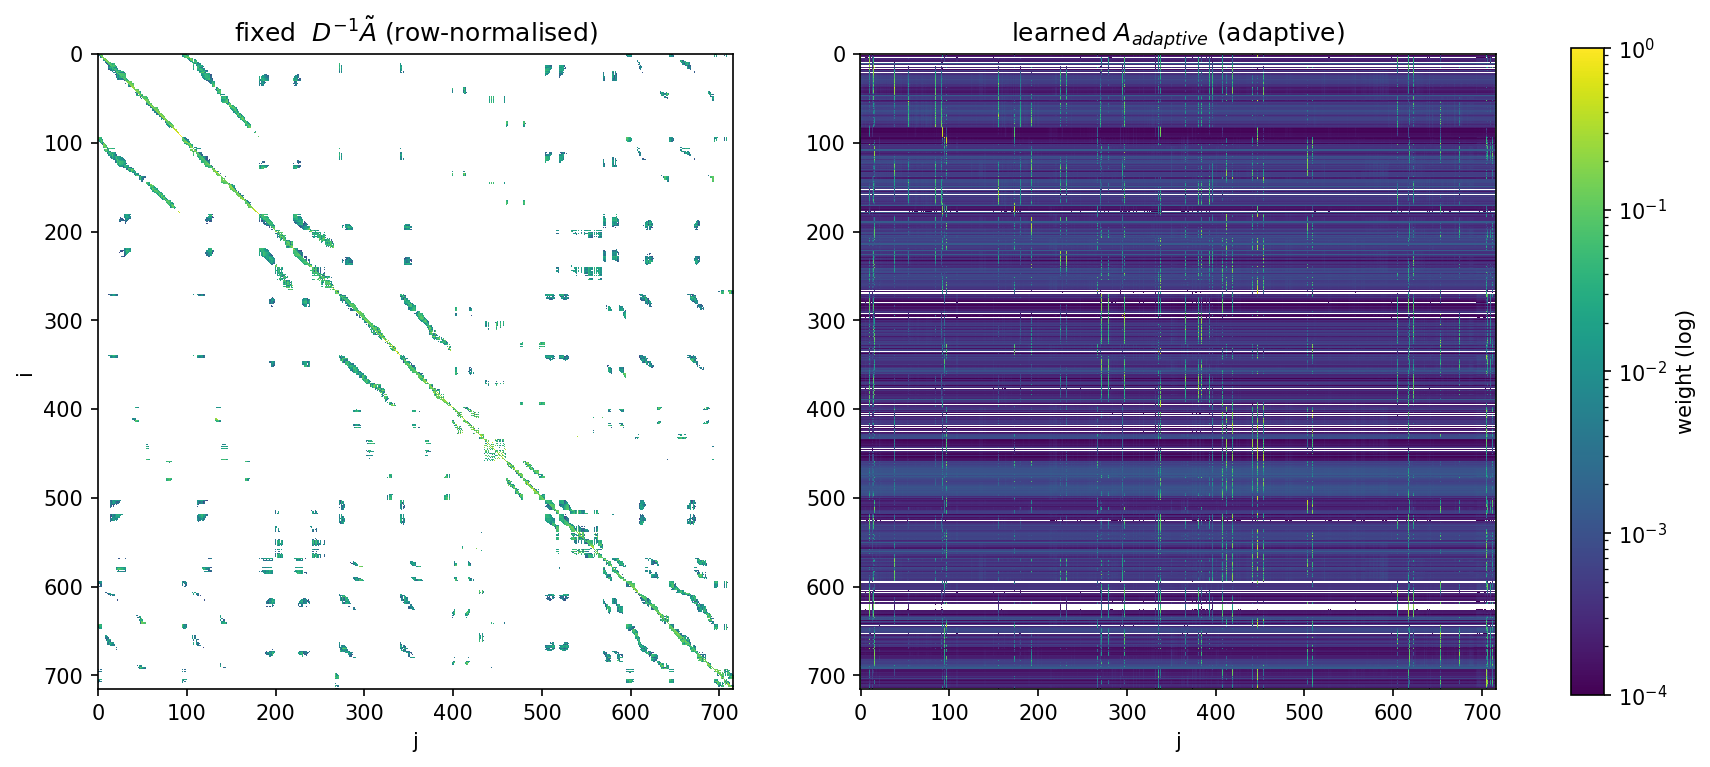
\includegraphics[width=\textwidth]{q5b_learned_adj_adaptive.png}
\caption{Left: fixed $D_{\text{out}}^{-1}\tilde A$. Right: learned $A_{\text{adaptive}}$ (as specified), same log colour scale, same sensor
order. The road graph is sparse and block-diagonal along freeways; the learned graph is dense and dominated by vertical stripes,
i.e.\ a few ``hub'' sensors that almost every row attends to.}\label{fig:adj}
\end{figure}
\begin{figure}[H]\centering
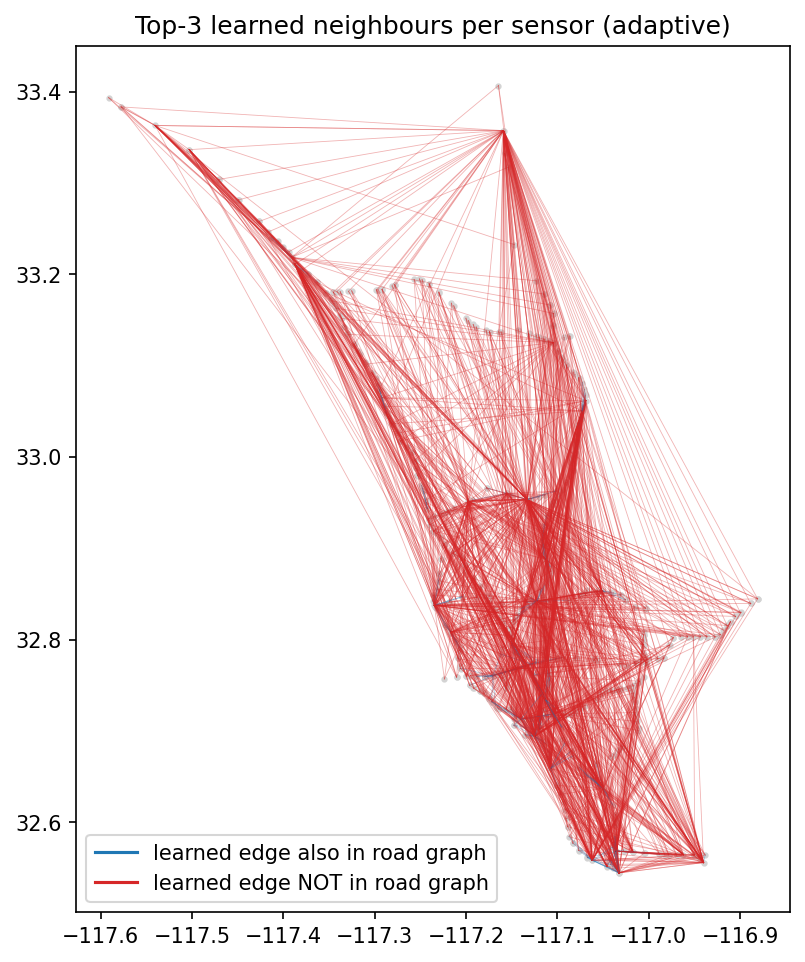
\includegraphics[width=.42\textwidth]{q6b_learned_edges_map_adaptive.png}\hfill
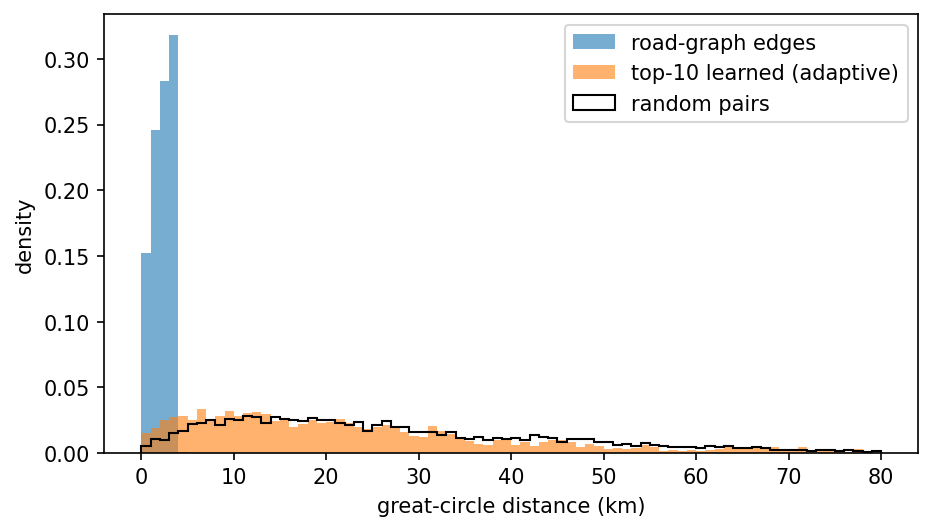
\includegraphics[width=.55\textwidth]{q6b_distance_adaptive.png}
\caption{Left: top-3 learned neighbours of every sensor on the map (blue: also a road-graph edge; red: not). Right: distance
distribution of road-graph edges, top-10 learned edges, and random sensor pairs.}\label{fig:map}
\end{figure}

\begin{enumerate}
\item \textbf{Are the strongest learned connections in the road graph?} Mostly not. Only 6.7\% of the top-10 learned edges are road
edges, though this is twice the random rate (3.4\%), and for the single strongest edge it is 16.6\% (5$\times$ random). On average the
model gives road-graph pairs 2.9$\times$ more weight than other pairs. So the road graph is visible in the learned matrix but it is not
the main structure (Fig.~\ref{fig:adj}): most of the weight goes to about 60 hub sensors (one sensor is in the top-10 of 263 rows).
\item \textbf{Do learned connections occur between nearby sensors?} No. The median top-10 learned edge is 19.8\,km long, close to the
23.1\,km of random pairs and far from the 2.4\,km of road edges; only 8.5\% are within 4\,km (Fig.~\ref{fig:map}). The model does not
learn a local neighbourhood.
\item \textbf{Does it capture dependencies absent from the physical graph?} Some, but not in the sense of ``similar commute'' pairs. Learned
edges outside the road graph link sensors whose changes are only slightly more correlated than random (0.078 vs 0.061). What the hubs
provide is mainly \emph{network-wide context}: a weighted average over a few representative sensors tells every node the current
state of the whole network (time of day, holiday, a city-wide drop), information a 4\,km road neighbourhood does not have. The
learned edges that \emph{are} road edges are the most correlated pairs of all (0.287 vs 0.172 for road edges on average), i.e.\ the model keeps the
physically strongest local links. Each row also has its own mixture (entropy 3.9 nats $\approx e^{3.9}\approx 50$ effective
neighbours), which the head can use to tell sensors apart.
\item \textbf{Why can a learned matrix be better or worse than the fixed one?}
\emph{Better}: it is optimised for the loss, can link distant sensors and use global context, can learn its own self-weights (instead of the fixed $1/\sum_j\tilde A_{ij}$), and is not limited by errors or the fixed 4\,km cut-off of the road graph. \emph{Worse}: it has
$N\cdot 2d_e$ extra parameters and no physical prior, so it can overfit or learn shortcuts, it costs $O(N^2)$ per step, and it is
static. In our runs the learned graph wins in both settings.
\end{enumerate}

\noindent\textbf{A collapse in the skip-connection runs.} In \texttt{adaptive\_res} and \texttt{hybrid\_res} every entry of $E_1E_2^\top$ ended up
$\le0$ (checked from the saved weights): $\mathrm{ReLU}$ then outputs 0 everywhere, the row softmax is exactly uniform ($1/716$, entropy
$=\ln716$), and no gradient reaches $E_1,E_2$ any more, so the graph cannot recover (a ``dead ReLU'' graph). The graph layer then computes
the same network mean $\frac1N\sum_jZ_jW_g$ for every node. Since the head also gets $Z_i$, this model is ``own history + global context'',
and it is the best one (test MAE 54.2). The hybrid model did the same and set $\lambda=0.04$. The skip connection removed the need
for the graph to carry the node's own signal, and the optimiser then preferred a global average over any specific structure. A top-$k$
or a $\mathrm{LeakyReLU}$/no-ReLU logit would avoid this collapse; I report the runs as they are, because they show clearly what the gains
in Table~\ref{tab:main} come from.

\subsection*{(c) Critical discussion}
\textbf{Does lower error mean the learned graph is the road network?} No, and our results show it directly. The best model
(adaptive, with skip, MAE 54.2) uses an exactly uniform graph, which has no connectivity information at all, and beats the real road graph
(59.8). Without the skip connection the learned graph is better than the road graph by 62 MAE while only 6.7\% of its strongest edges are
roads. A learned adjacency is whatever weighting of other sensors' features reduces the loss: hubs that summarise the network,
correlations caused by the shared daily cycle rather than by flow between sensors, or compensation for weaknesses of the rest of
the architecture (here, the lack of a self-path). Accuracy measures whether the graph is \emph{useful}, not whether it is \emph{true}. To
claim it reflects road structure one would need to test against the road graph (as in Table~\ref{tab:graph}), check stability over seeds,
and test interventions (e.g.\ closures).

\textbf{Why might a hybrid outperform either alone?} The two graphs carry different information: the road graph is a reliable,
sparse prior for \emph{local} propagation (upstream/downstream, ramps) that costs no parameters and works for sensors with little data,
while the adaptive graph adds what the road graph misses: long-range and network-wide dependencies and a learned self-weight. The mixture
can use local physics where it is reliable and data-driven structure elsewhere, and the prior regularises the learned part (less
overfitting, more stable training, a sensible graph from the first epoch). With $\lambda$ learned, the model can also choose the
balance: as specified it keeps $\lambda=0.35$ and is the best of the three graph models (MAE 78.9 vs 79.7 adaptive and 142.2
fixed). With the skip connection $\lambda\to0.04$ and hybrid $\approx$ adaptive, i.e.\ the hybrid is never worse than the better of the
two by more than noise, because it can always fall back to one of them.

\textbf{Limitations of a static graph.} Traffic dependencies change with time: in free flow, influence travels downstream at vehicle
speed; in congestion, shock waves travel \emph{upstream}, so the useful direction reverses. Which neighbours matter differs between the AM and
PM peaks (opposite commuting directions), weekdays and weekends, and during incidents, roadworks, closures and events, and the spatial
range of influence grows with the horizon and shrinks in congestion. A single static $\hat A$, fixed or learned, can only represent an
average over all these regimes; the uniform ``global average'' graph we obtained is an extreme case. Static graphs also cannot
adapt to sensors failing (they keep giving weight to a missing sensor). Remedies are time-varying or input-dependent adjacency
(attention over neighbours computed from the current window, e.g.\ GAT or graph WaveNet-style dynamic graphs), separate graphs per time
of day, or adding time-of-day/day-of-week features so the same graph can be used differently in different regimes.

%=====================================================================
\section*{Question 7 -- Reproducibility and reporting}

\textbf{Code and instructions.} \url{https://github.com/Awais65/DL4STG-PA3}. \texttt{README.md} lists the commands; in short:
\begin{lstlisting}
pip install -r requirements.txt                    # Python 3.10, PyTorch 2.6
python src/prepare_data.py --raw <LargeST folder>  # Q3a/b -> data/processed/
python src/q1_aggregation.py; python src/q2_ring.py; python src/q3_analysis.py
bash run_all.sh                                    # Q4/Q5: 8 runs, seed 42
python src/q6_analysis.py                          # Q6 tables, plots, graph analysis
\end{lstlisting}
Per-run outputs are \texttt{results/<tag>.json} (config, every epoch's metrics, timing, hardware) and \texttt{results/logs/<tag>.log}.

\textbf{Hyperparameters.}
\begin{center}\small
\begin{tabular}{ll}\toprule
Input / output & 8 steps (2\,h) $\to$ 4 steps (1\,h), $N=716$, $F=1$\\
Hidden dimension $d$ & 32 (encoder, graph conv, head)\\
Node embedding $d_e$ & 10 (adaptive/hybrid); dense, no top-$k$\\
Hybrid $\lambda$ & $\sigma(\theta)$, learned, initialised at 0.5\\
Loss & masked MAE in original units (observed targets only)\\
Optimiser & Adam, lr $10^{-3}$, weight decay $10^{-4}$, gradient clip 5\\
LR schedule & ReduceLROnPlateau on val MAE, factor 0.5, patience 3\\
Batch size & 64 windows\\
Epochs & max 50, early stopping on val MAE with patience 8; best checkpoint used\\
Epochs run (best) & see Table~\ref{tab:main}\\
Random seed & 42 (Python, NumPy, PyTorch, CUDA); cuDNN deterministic\\\bottomrule
\end{tabular}
\end{center}

\textbf{Hardware and training time.} Laptop with Intel Core i9-14900HX (24 cores / 32 threads), 32\,GB RAM, NVIDIA GeForce RTX 4070
Laptop GPU (8\,GB, driver 577.02), Windows 11; Python 3.10.19, PyTorch 2.6.0 (CUDA 12.4), NumPy 2.2.6. All runs used the GPU and
were run one after another so the times are comparable. Measured training time (wall clock, all epochs including validation) is in
Table~\ref{tab:main}: 316--377\,s per model, 6.3--7.5\,s per epoch, about 47\,min for all eight runs. The models are small (9.6k--24k
parameters), so they also train on a CPU, more slowly.

\textbf{Required items.} Source code and instructions: repository above. Hyperparameters, epochs, seed: table above and Table~\ref{tab:main}.
Final comparison table: Table~\ref{tab:main}. Adjacency visualisations: Q3(b) and Fig.~\ref{fig:adj}. Predicted vs.\ actual plots:
Figs.~\ref{fig:pred1}--\ref{fig:pred2}. Hardware and training times: this section.

%=====================================================================
\section*{Use of generative AI}
As allowed by the course AI policy, I used \textbf{Claude Code} (Anthropic's AI coding assistant, model Claude Opus, running in my
terminal with access to the PA3 folder) for this assignment. It wrote the code, ran the experiments and drafted the report text;
the full session transcripts are saved by the tool and can be provided on request. Below are all the prompts I gave, verbatim
(including typos), in order, with what the tool produced and the edits made.

\begin{enumerate}[leftmargin=*]
\item \textbf{Session 1 (17 Nov 2026)} -- \textbf{Prompt:} ``review the contents of PA3''.\\
\textbf{Output:} a summary of the assignment PDF: deadline and late policy, the requirement for a public GitHub repository and this
AI-use section, a per-question breakdown of the tasks and effort, and risks (Q3 data size being the critical path).
\textbf{Edits:} none (information only).

\item \textbf{Session 2 (20 Nov 2026)} -- \textbf{Prompt:} ``lets start with PA3''.\\
\textbf{Output:} from this single prompt the tool did most of the work, checking each step numerically:
\begin{itemize}
\item Q1 and Q2: wrote \texttt{src/q1\_aggregation.py} and \texttt{src/q2\_ring.py}, derived the answers and verified them in NumPy
(e.g.\ the 164-neighbourhood brute-force checks, the least-squares fit $a=0,b=\tfrac12$, the $[0,0,1]$ kernel and $a=0,b=1,c=-1$).
\item Q3: downloaded LargeST from Kaggle, wrote \texttt{src/prepare\_data.py} (SD extraction by sensor ID, summing 5-min counts to
15-min after checking the values are integer counts, missing-value handling using training statistics only, adjacency extraction)
and \texttt{src/q3\_analysis.py} (statistics, figures, neighbourhoods, neighbour correlations).
\item Q4/Q5: wrote \texttt{src/models.py} and \texttt{src/train.py} (temporal encoder, graph convolution, head; fixed directed
row-normalised, adaptive and hybrid adjacency; masked MAE). It chose the directed normalisation $D_{\text{out}}^{-1}\tilde A$
because the graph is not symmetric, and proposed the skip-connection runs as an extra, clearly labelled comparison
because it expected the specified layer to dilute each sensor's own features.
\item Wrote the Q1--Q3 sections of this report, \texttt{README.md}, \texttt{requirements.txt} and \texttt{run\_all.sh}, and started training.
\end{itemize}
\textbf{Edits:} the training run started in this session was interrupted before finishing and was re-run from scratch in session 3.

\item \textbf{Session 2} -- \textbf{Prompt:} ``let me setup the git what should be the repo name''.\\
\textbf{Output:} a suggested name and the git commands. \textbf{Edits:} I did not use the suggested name; I named the repository
\texttt{DL4STG-PA3} to match my PA1 and PA2 repositories (session 3, below).

\item \textbf{Session 3 (20 Nov 2026)} -- \textbf{Prompts:} ``check screenshot for previous git repo name so we can name third one
accordingly'', ``check the assignment instruction i think its public'', the repository URL, ``its public repo''.\\
\textbf{Output:} it found my PA1/PA2 repository names, confirmed from the PDF that the repository must be public, initialised git,
committed the project and set the remote. I created the public repository on GitHub and pushed it myself.
It then inserted the repository link on the first page of this report.

\item \textbf{Session 3} -- \textbf{Prompts:} ``compile the report pdf'', ``is it complete?'', ``yes start training and finish the rest'',
``how long left on training?''.\\
\textbf{Output:} it found that the report did not compile (the Q4--Q7 file was missing) and that training had stopped, re-ran all
eight training runs (\texttt{run\_all.sh}) and \texttt{src/q6\_analysis.py}, added predicted-vs-actual plots for the skip-connection
models to \texttt{q6\_analysis.py}, inspected the saved embeddings (finding the dead-ReLU collapse reported in Q6b), wrote the
Q4--Q7 sections and the hardware details, and compiled the PDF.\\
\textbf{Edits:} before finalising, the tool checked its draft against the data and corrected two claims that were wrong:
the fixed graph's self-weight (median 0.14, not $\approx$0.04 as first written) and an unsupported claim that the test
period had more missing data (it has the same fraction as validation; the error gap is explained by higher flow levels instead).
It also removed an unverified statement about the ranking being stable, and fixed table widths.

\item \textbf{Session 3} -- \textbf{Prompt:} ``fill in the AI usage section for me''.\\
\textbf{Output:} this section, written from the saved session transcripts.
\end{enumerate}

\noindent The design choices in this report (summing counts, the directed normalisation, reporting both the as-specified and skip-connection
models, and reporting the collapsed adaptive graph as it is) were proposed by the tool and accepted by me. I have read the report and
can explain each part.
